%\documentclass[10pt, handout]{beamer}
\documentclass[10pt]{beamer}
% use the first one to ignore /pause and the second one to make use of it!
\usetheme[
%%% option passed to the outer theme
%    progressstyle=fixedCircCnt,   % fixedCircCnt, movingCircCnt (moving is deault)
  ]{Feather}
  
% If you want to change the colors of the various elements in the theme, edit and uncomment the following lines

% Change the bar colors:
%\setbeamercolor{Feather}{fg=red!100,bg=red!0}

% Change the color of the structural elements:
\setbeamercolor{structure}{fg=white}

% Change the frame title text color:
\setbeamercolor{frametitle}{fg=white}

% Change the normal text color background:
\setbeamercolor{normal text}{fg=white, bg= }%gray!90}

\definecolor{light-gray}{gray}{0.7}

%-------------------------------------------------------
% INCLUDE PACKAGES
%-------------------------------------------------------

\usepackage[utf8]{inputenc}
\usepackage[ngerman]{babel}
\usepackage[T1]{fontenc}
\usepackage{helvet}
\usepackage{array}

\usepackage{pdfpages}

\usepackage{listings}
%\usepackage{tikz}
%\usepackage{tkz-graph}
%\usetikzlibrary{calc}
%\usetikzlibarary{calc}

%-------------------------------------------------------
% DEFFINING AND REDEFINING COMMANDS
%-------------------------------------------------------

% colored hyperlinks
\newcommand{\chref}[2]{
  \href{#1}{{\usebeamercolor[bg]{Feather}#2}}
}

%-------------------------------------------------------
% INFORMATION IN THE TITLE PAGE
%-------------------------------------------------------

\title[Lego Car] % [] is optional - is placed on the bottom of the sidebar on every slide
{ % is placed on the title page
      \textbf{Lego Car}
}

\subtitle[Midterm Presentation]
{
      \textbf{Midterm Presentation}
}

\author[Autor]
{      
	Berkay, Moritz Dötterl, Abdallah, Heiko Lengenfelder TODO: Nachnamen eintragen
}

%\institute[]
%{
%       "Estar no estado de graça concede ao homem o céu no futuro; saber que está no estado de graça concede o céu agora e no futuro". - Thomas Brooks (Livro "Céu na Terra" de 1654)
  
  %there must be an empty line above this line - otherwise some unwanted space is added between the university and the country (I do not know why;( )
%}

\date{30.5.2016}


%-------------------------------------------------------
% THE BODY OF THE PRESENTATION
%-------------------------------------------------------



\begin{document}

%-------------------------------------------------------
% THE TITLEPAGE
%-------------------------------------------------------

{\1% % this is the name of the PDF file for the background
\begin{frame}[plain,noframenumbering] % the plain option removes the header from the title page, noframenumbering removes the numbering of this frame only
  \titlepage % call the title page information from above
\end{frame}

{
\addtobeamertemplate{navigation symbols}{}{%
    \usebeamerfont{footline}%
    \usebeamercolor[fg]{title}%
    \hspace{5em}%
   \normalsize\insertframenumber/\inserttotalframenumber
}
\begin{frame}[plain]{\huge Agenda}
	\begin{itemize}
	\LARGE
		\item Nano Board
		\item Wiring
		\item Raspberry Pi
		\item OpenCV
	\end{itemize}

\end{frame}


}

\includepdf[pages=-]{berkay.pdf}
{\1
 
\begin{frame}[plain]{Wiring}{overview}
	Components:
	\center
	\pause
	\begin{itemize}
		\item Sensors
		\begin{itemize}
			\item Ultrasonic
			\item Camera
		\end{itemize}
		\pause
		\item Actuators
		\begin{itemize}
			\item Steering Servo
			\item Drive Motor
		\end{itemize}
		\pause
		\item Controll
		\begin{itemize}
			\item Nanoboard
			\item Raspberry Pi
		\end{itemize}
		\pause
		\item Power supply
		\begin{itemize}
			\item Battery
			\item H-Bridge
		\end{itemize}
	\end{itemize}
	
\end{frame}
 
 
 \begin{frame}[plain]{Wiring}{circuit layout}
	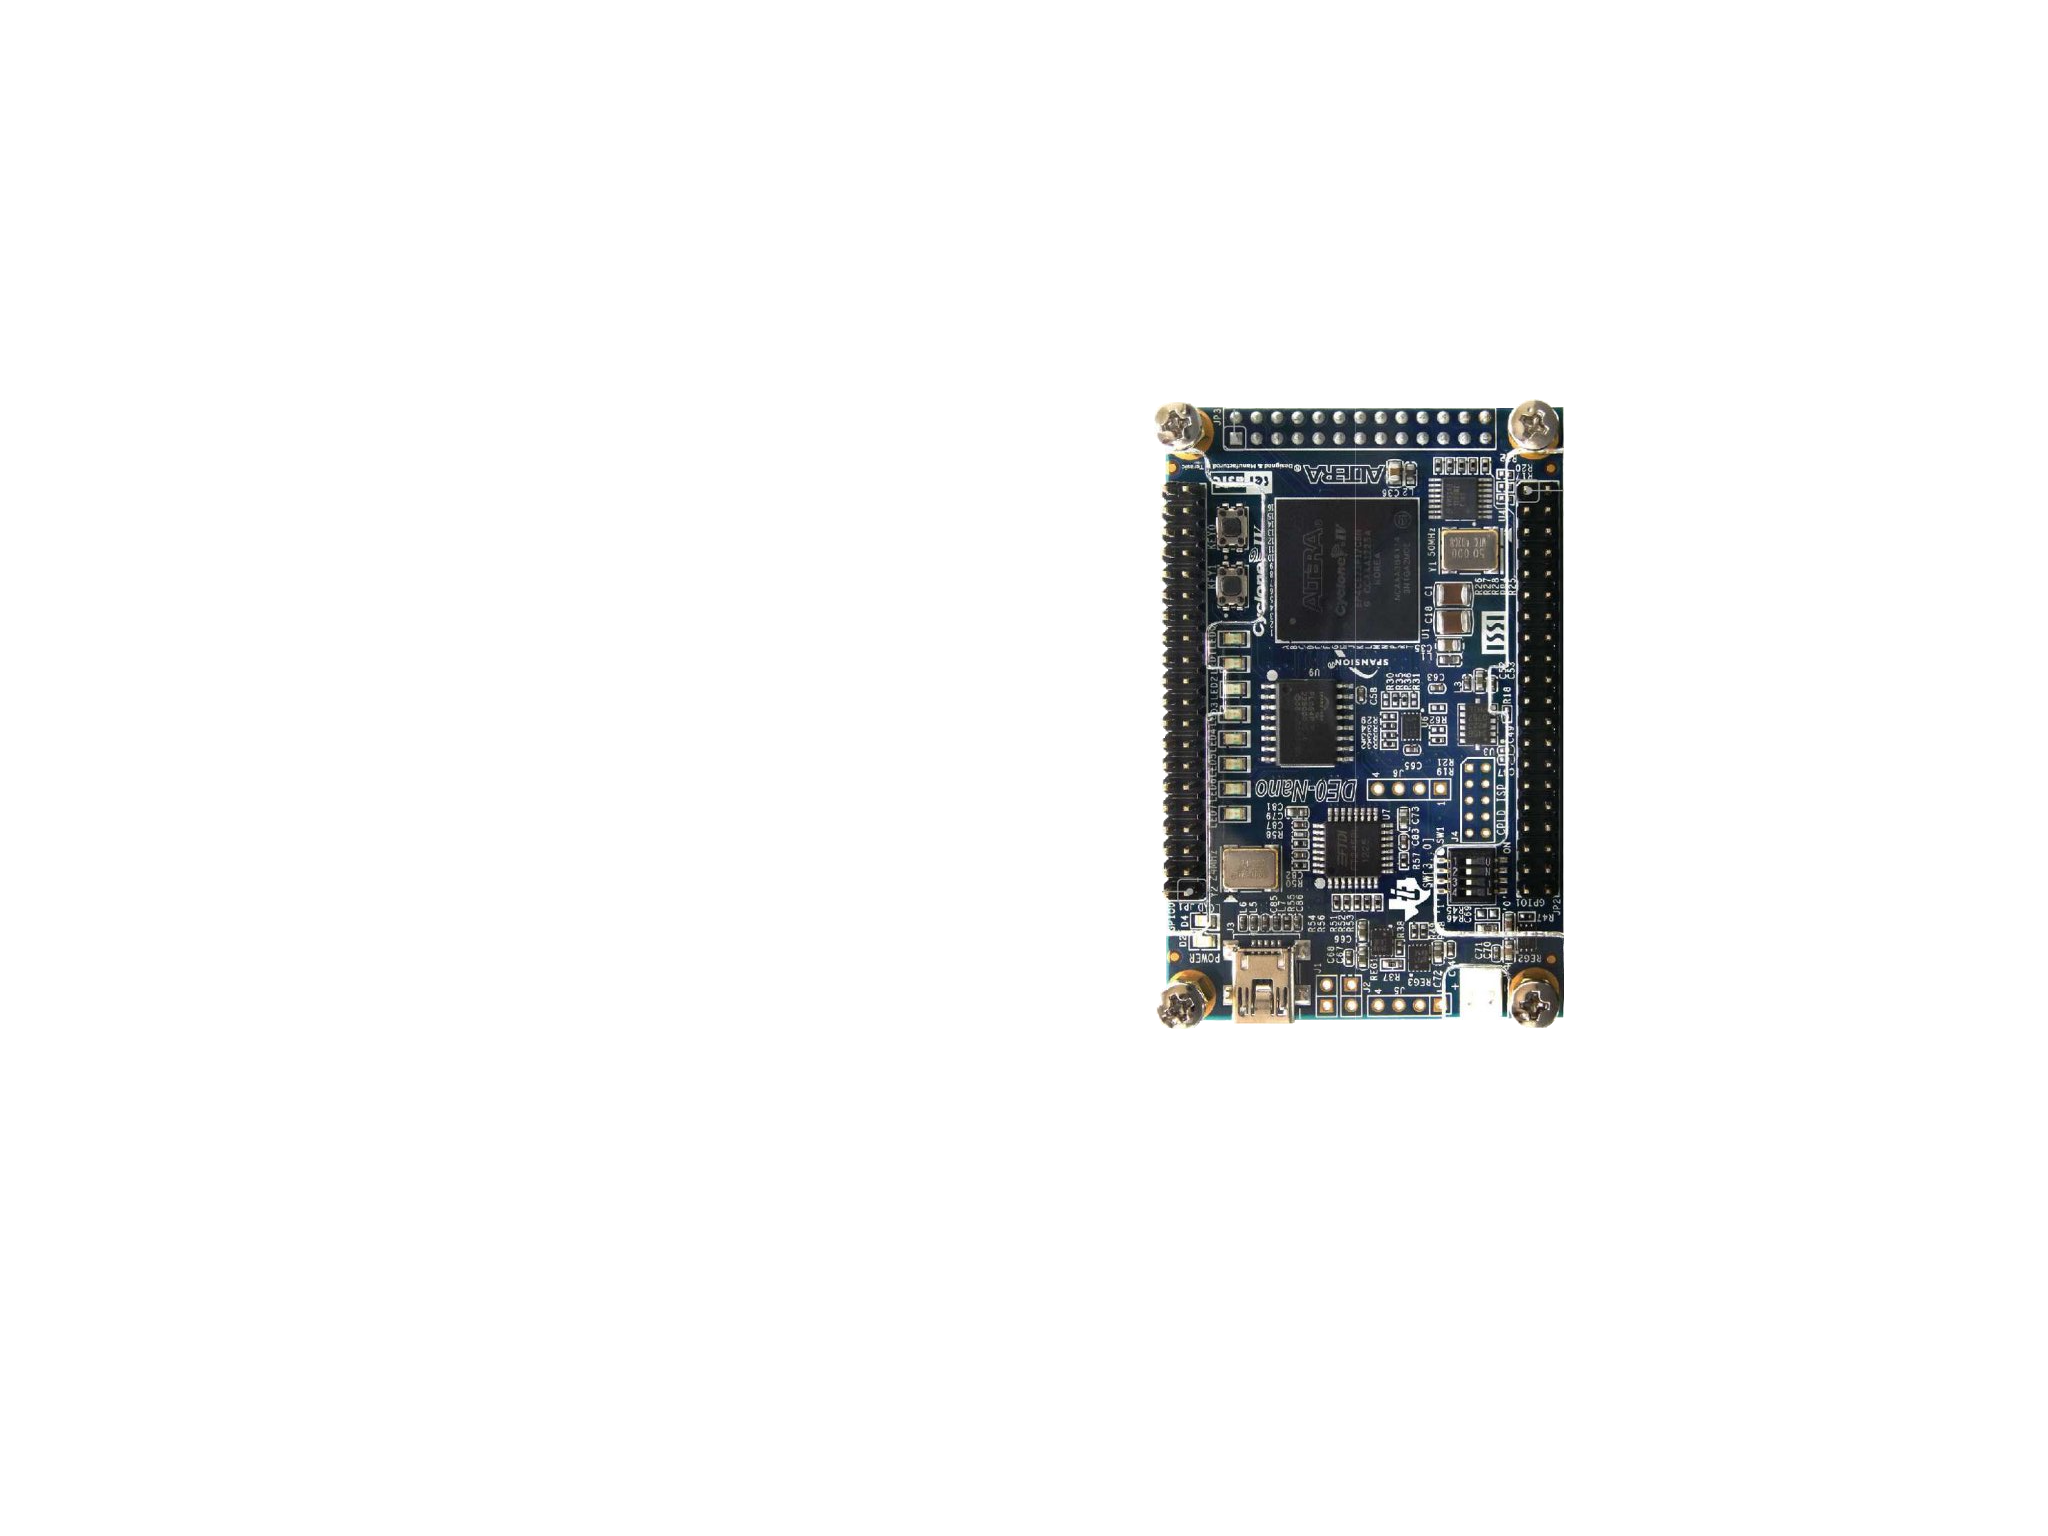
\includegraphics[width=\textwidth]{Feathergraphics/wiring1}
	\end{frame}
	
	
 \newcounter{ctra}
\setcounter{ctra}{2}
\whiledo {\value{ctra} < 13}%
{%
\begin{frame}[plain,noframenumbering]{Wiring}{circuit layout}
	\includegraphics[width=\textwidth]{Feathergraphics/wiring\the\value{ctra}}

\end{frame}
 \stepcounter {ctra}%
}
\addtocounter{page}{-16}
 
\begin{frame}[plain]{Raspberry Pi}
	% this is a comment
	\begin{itemize}
		\item Raspberry Pi Version: Raspberry Pi 3
		\item Capable little computer that can be used for electronics projects
		\item Used to connect the camera with the nano-board for the line detection
	\end{itemize}
	
	\begin{figure}
	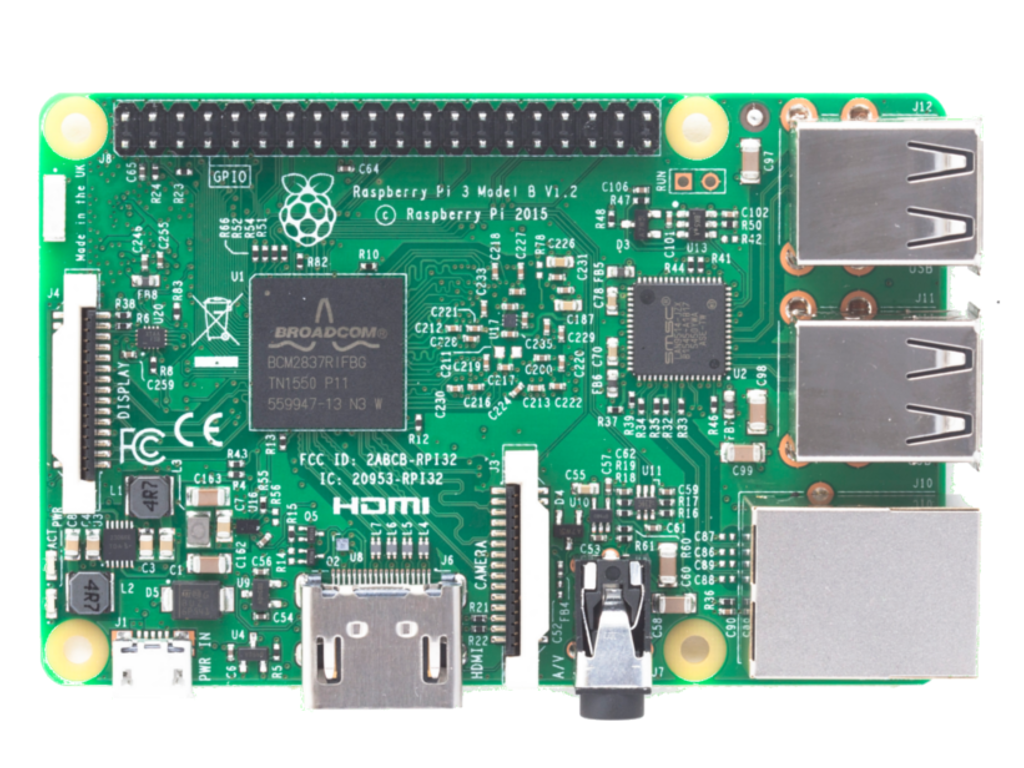
\includegraphics[width=7cm, height=5cm]{raspi2.png}
	\end{figure}
	
	\vspace{2cm}
	this text has 2cm Distance from above (because of vspace)\\ % \\ means new line
	Abdallah
\end{frame}

\begin{frame}[plain]{Raspberry Pi}

Carried out steps:
\begin{enumerate}
		\item Raspbian installed (operating system for the Raspberry Pi)
		\item Connected to the laptop using Ethernet
		\item Used SSH (Secure Shell) to gain access to the command line of the Raspberry Pi
		\item Controlled the Raspberry Pi using VNC (a graphical desktop sharing system)
		\item Downloaded OpenCV and connected the camera
		\item Tested the Code for the line detection
	\end{enumerate}
	

	
To-Do:
\begin{enumerate}
		\item Connect the Raspberry Pi to the nano-board
		\item Align the line detection with the motor control
	\end{enumerate}

\end{frame}

\begin{frame}[plain]{Raspberry Pi}
\begin{figure}
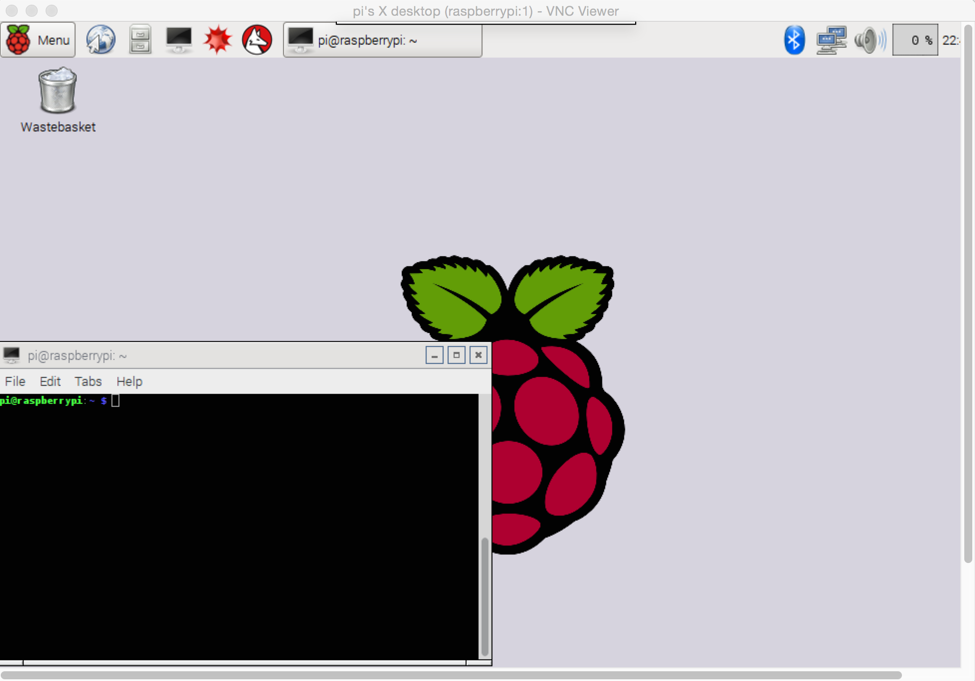
\includegraphics[width=8cm, height=7cm]{vnc.png}
\end{figure}	
\end{frame}
 
\begin{frame}[plain]{Line Detection}
	% this is a comment
	Approach
	\begin{itemize}
		\item Approximate line
		\item Calculate direction
	\end{itemize}
	\pause
	Assumptions
	\begin{itemize}
		\item Vertical line
		\item Car position
		\item Line is highest contrast on image
		\item Width of line (optional)
	\end{itemize}
\end{frame}	

\begin{frame}[plain]{Line Detection}
	\begin{columns}[T]
		\begin{column}[T]{5cm}
			\vspace{5mm}
			Steps
			\begin{itemize}				
				\visible<1->{\item Get Frame from camera}
				\visible<2->{\item Apply Gaussian Filter}
				\visible<3->{\item Transform image from RGB to grey}
				\visible<4->{
				\item Approximate Gradient
					$
					M=
					\begin{bmatrix}
					-1 & 0 & 1 \\
					-2 & 0 & 2 \\
					-1 & 0 & 1
					\end{bmatrix}
					$			
				}
				\visible<5->{\item Calculate maximal points for each row}
				\visible<6->{\item Fit line on points}
				\visible<7->{\item Calculate direction of car}
			\end{itemize}
		\end{column}
		\begin{column}[T]{7cm}
			\vspace{1cm}
			\includegraphics<1>[width=\textwidth]{Heikographics/line1}
			\includegraphics<2>[width=\textwidth]{Heikographics/line2}
			\includegraphics<3>[width=\textwidth]{Heikographics/line3}
			\includegraphics<4>[width=\textwidth]{Heikographics/line4}
			\includegraphics<5>[width=\textwidth]{Heikographics/line5}
			\includegraphics<6>[width=\textwidth]{Heikographics/line6}
			\includegraphics<7>[width=\textwidth]{Heikographics/line7}
		\end{column}
	\end{columns}
\end{frame}


\begin{frame}[plain]{Line Detection}
	Pros/Cons
	\begin{itemize}
		\item Fast calculation time
		\item Vulnerable to noise
	\end{itemize}
	TODO
	\begin{itemize}
		\item Calculate discrete angle
		\item Attaching camera
		\item Testing/Optimization
	\end{itemize}
\end{frame}
}
}

\end{document}
